\documentclass[spanish,12pt]{article}
\usepackage[spanish]{babel}
\usepackage[utf8]{inputenc}
\usepackage{xspace}
\usepackage{lmodern}
\usepackage{indentfirst}
\usepackage{xargs}
\usepackage{ifthen}
\usepackage{fancyhdr}
\usepackage{latexsym}
\usepackage{lastpage}
\usepackage{textcomp}
\usepackage{varwidth}
\usepackage{caratula, aed2-tad,aed2-symb,aed2-itef}
\usepackage{algorithmicx, algpseudocode, algorithm}
\usepackage{enumerate}
\usepackage{graphicx}
\usepackage{caption}
\usepackage{subcaption}
\usepackage{float}
\usepackage{anysize}
\marginsize{1.5cm}{1.5cm}{1.5cm}{1.5cm}

\begin{document}

\titulo{Informe 2}
\materia{Algoritmos y Estructuras de Datos III}
\author{Grupo  \\Alvarez Vico Jazm\'in\\Cortés Conde Titó Javier María\\Pedraza Marcelo \\ Rozenberg Uriel Jonathan}

\integrante {Jazmín Alvazer Vico}{75/15}{jazminalvarezvico@gmail.com}
\integrante {Marcelo Pedraza}{393/14}{marcelopedraza314@gmail.com}
\integrante {Uriel Jonathan Rozenberg}{838/12}{rozenberguriel@gmail.com}
\integrante {Javier María Cortés Conde Titó}{252/15}{javiercortescondetito@gmail.com}

\maketitle


\clearpage

\tableofcontents
\cleardoublepage

\section{Problema 1: }

\subsection{Introducción}


%terminar?%

\subsection{Explicación de la solución}


%creeeo que le falta%



\subsection{Pseudocódico}


\subsection{Demostración de Correctitud}



\subsection{Demostración de Complejidad}


\subsection{Experimentación}

%%%%%%%%%%%%%%%%%%%%%%%%%%%%%%%%%%%%%%%%%%%%%%%%%%%

\section{Problema 2: }

\subsection{Introducción}


\subsection{Explicación de la solución}



\subsubsection{Pseudocódigo}


\subsubsection{Demostración de Correctitud}


\subsubsection{Demostración de Complejidad}


\subsection{Experimentación}


\subsubsection{Análisis complejidad te\'orica}


\subsubsection{Análisis}



\section{Problema 3: Escapando}

\subsection{Introducción}

En este problema, los exploradores se encuentran en un dilema, luego de romper varias paredes la fortaleza se esta derrumbando. Por suerte ellos se encuentran en una habitación que tiene varios carritos y un mapa que les indica que estaciones estan conectadas y cuanto tardan en llegar de estación a estación. Lo que quieren es la forma más rápida de llegar desde el lugar en donde estan hasta la salida, que seria la ultima estación.

Formalmente, tenemos un digrafo rotulado, con peso en los ejes, y cada nodo esta identificado por un número desde el uno hasta la cantidad de nodos. Nuestro objetivo es encontrar el camino mínimo, dando el tiempo y su conjunto de ejes.


\subsection{Explicación de la solución}

   En esta sección explicaremos por que el problema dado se puede adapatar al algoritmo de camino mínimo de Dijkstra.
 Las precondiciones que el algoritmo de Dijkstra pide es que no tenga ejes negativos. Como el peso de los ejes esta definido como el tiempo que se tarda de llegar del nodo de origen al nodo de llegada podemos asegurarnos que nunca vamos a tener una entrada, que nos importe, tal que exista un eje con peso negativo. 

\subsubsection{Pseudocódigo}

\begin{algorithm}[H]{\textbf{CaminoMinimo}(MatrizAdy: Matriz(Nat, Nat) , estaciones: vector$<$Nat$>$)}
	\begin{algorithmic}[1]
		
		\State n $\gets$ tamaño(MatrizAdy)
		\State NodosSeguros $\gets$ 1
		\State nodosNoSeguros $\comment$ conjunto $\{$2, ..., n$\}$
		\State mientras NodosSeguros $\neq$ G
		\State \quad nodomin $\gets$ buscarMin(nodos, MatAdy[1])
		\State \quad nodosNoSeguros - $\{$nodomin$\}$
		\State \quad NodosSeguros $\cup$ $\{$nodomin$\}$
		\State \quad \forall \ e \ $\in$ nodos $\land$ [nodomin, e] $\in$ X
		\State \qquad longi $\gets$ $\pi_{1}$(matAdy[1][e])
		\State \qquad longmin $\gets$ $\pi_{1}$(matAdy[1][nodomin])
		\State \qquad longimin $\gets$ $\pi_{1}$(matAdy[nodomin][pos])
\\
		\qquad \textbf{if} longi $\geq$ longmin +longimin
			\State \qquad \quad matAdy[1][e] $\gets$ (longpmin + longimin, nodomin)
\\		 
 \qquad \textbf{endif}

		\State tiempo $\gets$ $\pi_{1}$(MatAdy[1][n])
		\State pred $\gets$ n
		\State mientras pred $\neq$ 1 \ $\land$ \ pred $\neq$ 0 (cuando no existe camino)
		\State \quad estaciones $\cup$ $\{$pred$\}$
		\State \quad pred $\gets$ $\pi_{2}$(matAdy[1][pred])

		\State res $\gets$ tiempo
 	\end{algorithmic}
\end{algorithm}

\begin{algorithm}[H]{\textbf{CaminoMinimo}(mochilas: vector$<$mochila$>$, cofre: vector$<$tesoro$>$)}
	\begin{algorithmic}[1]
		
		\State sol$\gets$ ValorOptim
	\end{algorithmic}
\end{algorithm}

\newpage

\subsubsection{Demostración de Correctitud}
Como podemos apreciar el pseudocódigo es el algoritmo Dijsktra, entonces su correctitud se desprende de la demostración de correctitud de dijkstra que se puede encontrar en varios libros de algoritmos, en nuesro caso vamos a referenciar al libro titulado "Introduction to Algorithms, Second Edition" de Thomas H Cormen, Charles E. Leiserson, entre otros. La demostracion se encientra en el capítulo 24, subsection 3 bajo el título "Theorem 24.6: (Correctness of Dijkstra's algorithm)". 

\subsubsection{Demostración de Complejidad}

%No pude tabular, ni con \quad ni con \tab ni con $\>$ ni con $\-$ pero parece ser un problema de el salto de linea.
Si analizamos con atención el pseudocódigo, Tenemos tres secciones que se pueden analizar por separado y despues sumar sus complejidades nos dara la complejidad total del algoritmo. La primer parte y la segunda parte combinadas son Dijkstra, la primera es la creación de la matriz y la segunda son los cálculos, La tercer parte es poner la información del camino mínimo. En los próximos párrafos nos vamos a referir a la cantidad de nodos en el gráfico como N. 
\\
	 La primer parte a analizar es la creación de la matriz, al ser una matriz de adyacencia, la cantidad de filas es N y la cantidad de columnas es N, actualizar todos los valores es recorrer toda la matriz haciendo que la complejidad sea $\Theta$(N²)
\\
	La segunda parte son dos ciclos anidados, podemos observar que el ciclo exterior hace N iteraciones ya que termina cuando el conjunto de nodos del grafo tiene el mismo cardinal que el conjunto de ``nodosSeguros'' y este último aumenta en uno por cada iteración. Dentro de el ciclo principal tenemos dos operaciones que debemos tener en cuenta, sacar el nodo de la lista de ``nodosNoSeguros'' y el ciclo interno. Sacar un nodo de la lista, nos va a costar encontrar el nodo y luego eliminarlo. Por la estructura que utlizamos eliminarlo no nos aporta complejidad, pero encontrar el nodo es una busqueda lineal, es decir $\mathcal{O}$(N). La última parte que nos falta analizar para poder determinar la complejidad de los ciclos anidados es el ciclo interno. Cada iteración recorre N posiciones de la matriz, aquellas que podrían ser un eje válido, aunque hace cosas dependiendo de si es un eje válido o no, el interior del cicclo aporta una complejidad constante. Reuniendo toda la informacion, el interior del ciclo externo nos aporta una complejidad $\mathcal{O}$(N) y itera N veces, es decir que la complejidad de la segunda parte es $\mathcal{O}$(N²).
\\
	 La tercer parte es un ciclo que lee los datos de la matriz y guarda en un conjunto los nodos que tenemos que atravezar para tener el camino mínimo. La cantidad máxima de iteraciones que hace este ciclo es N, el razonamiento atras de esta afirmación es que los ejes tienen pesos negativos, si existe un camino mínimo, este no va a tener ciclos ya que pasar por un ciclo solo aumentaría el peso total del camino, y un camino sin ciclos en un grafo con n nodos tiene como mucho n-1 ejes, ya que el camino puede llegar a pasar por todos los nodos. Podemos concluir que el ciclo hace n iteraciones en el peor caso, es Decir que la tercer parte es $\mathcal{O}$(N)
\\
\tab Ahora que analizamos las tres partes que podían llegar a dar complejidad al algoritmo sabemos que la complejidad algoritmica de la primer parte, la segunda parte y la tercera respectivamente son $\Theta$(N²), $\mathcal{O}$(N²), $\mathcal{O}$(N). Entonces la complejidad total es la suma de las complejidades dandonos $\mathcal{O}$(N²).

\subsection{Experimentación}

La cota de complejidad de nuestro algoritmo es $\mathcal{O}$(N²). Es decir que depende de la cantidad de nodos en un grafo.
En esta sección trataremos de respaldar esta cota mediante el análisis de los datos empíricos que obtuvimos a traves del testeo de nuestros algoritmos.
\\
Para clarificar nuestros algortimos son dos variaciones del pseudocódigo que mostramos, con la excepcion es que uno, el que decidimos usar para solucionar el problema deja de calcular en cuanto el nodo N se mete en la zona segura. Decidimos testear sobre los dos algoritmos ya que al asignar peso aleatorio a los ejes en la mayoría de los casos teníamos la intuición de que los gráficos podrían quedar bastante mal. Pensamos en hacer test donde nos asegurabamos que se recorrían todos los nodos, pero al final decidimos usar dos variaciones del mismo algoritmo para demostrar que el algoritmo que nosotros elejimos, en el peor caso tiene una complejidad igual al que realmente nos va a probar la cota N².
\\  
Con este objetivo a lo largo de los tests modificamos los inputs para observar de a una variable por vez dejando las otras constantes y así poder analizar el tiempo de ejecución en cada caso. En cada test los valores se logran al promediar un millón de iteraciones sobre el mismo input, sobre que forma tiene el input se va a hablar más adelante.

\subsubsection{Resultados y análisis}

En nuestro primer experimento fijamos una mochila con capacidad constante (50) y fuimos aumentando la cantidad de tesoros de a dos.
Así mismo, analizamos tres subcasos pertinentes: cuando los objetos están dados aleatoriamente (sin ninguna restricción sobre su peso), cuando el peso de los objetos se encuentra restringido a la capacidad de la mochila y cuando el peso de objetos es superior a la capacidad de la mochila.

\begin{figure}[H]
\centering
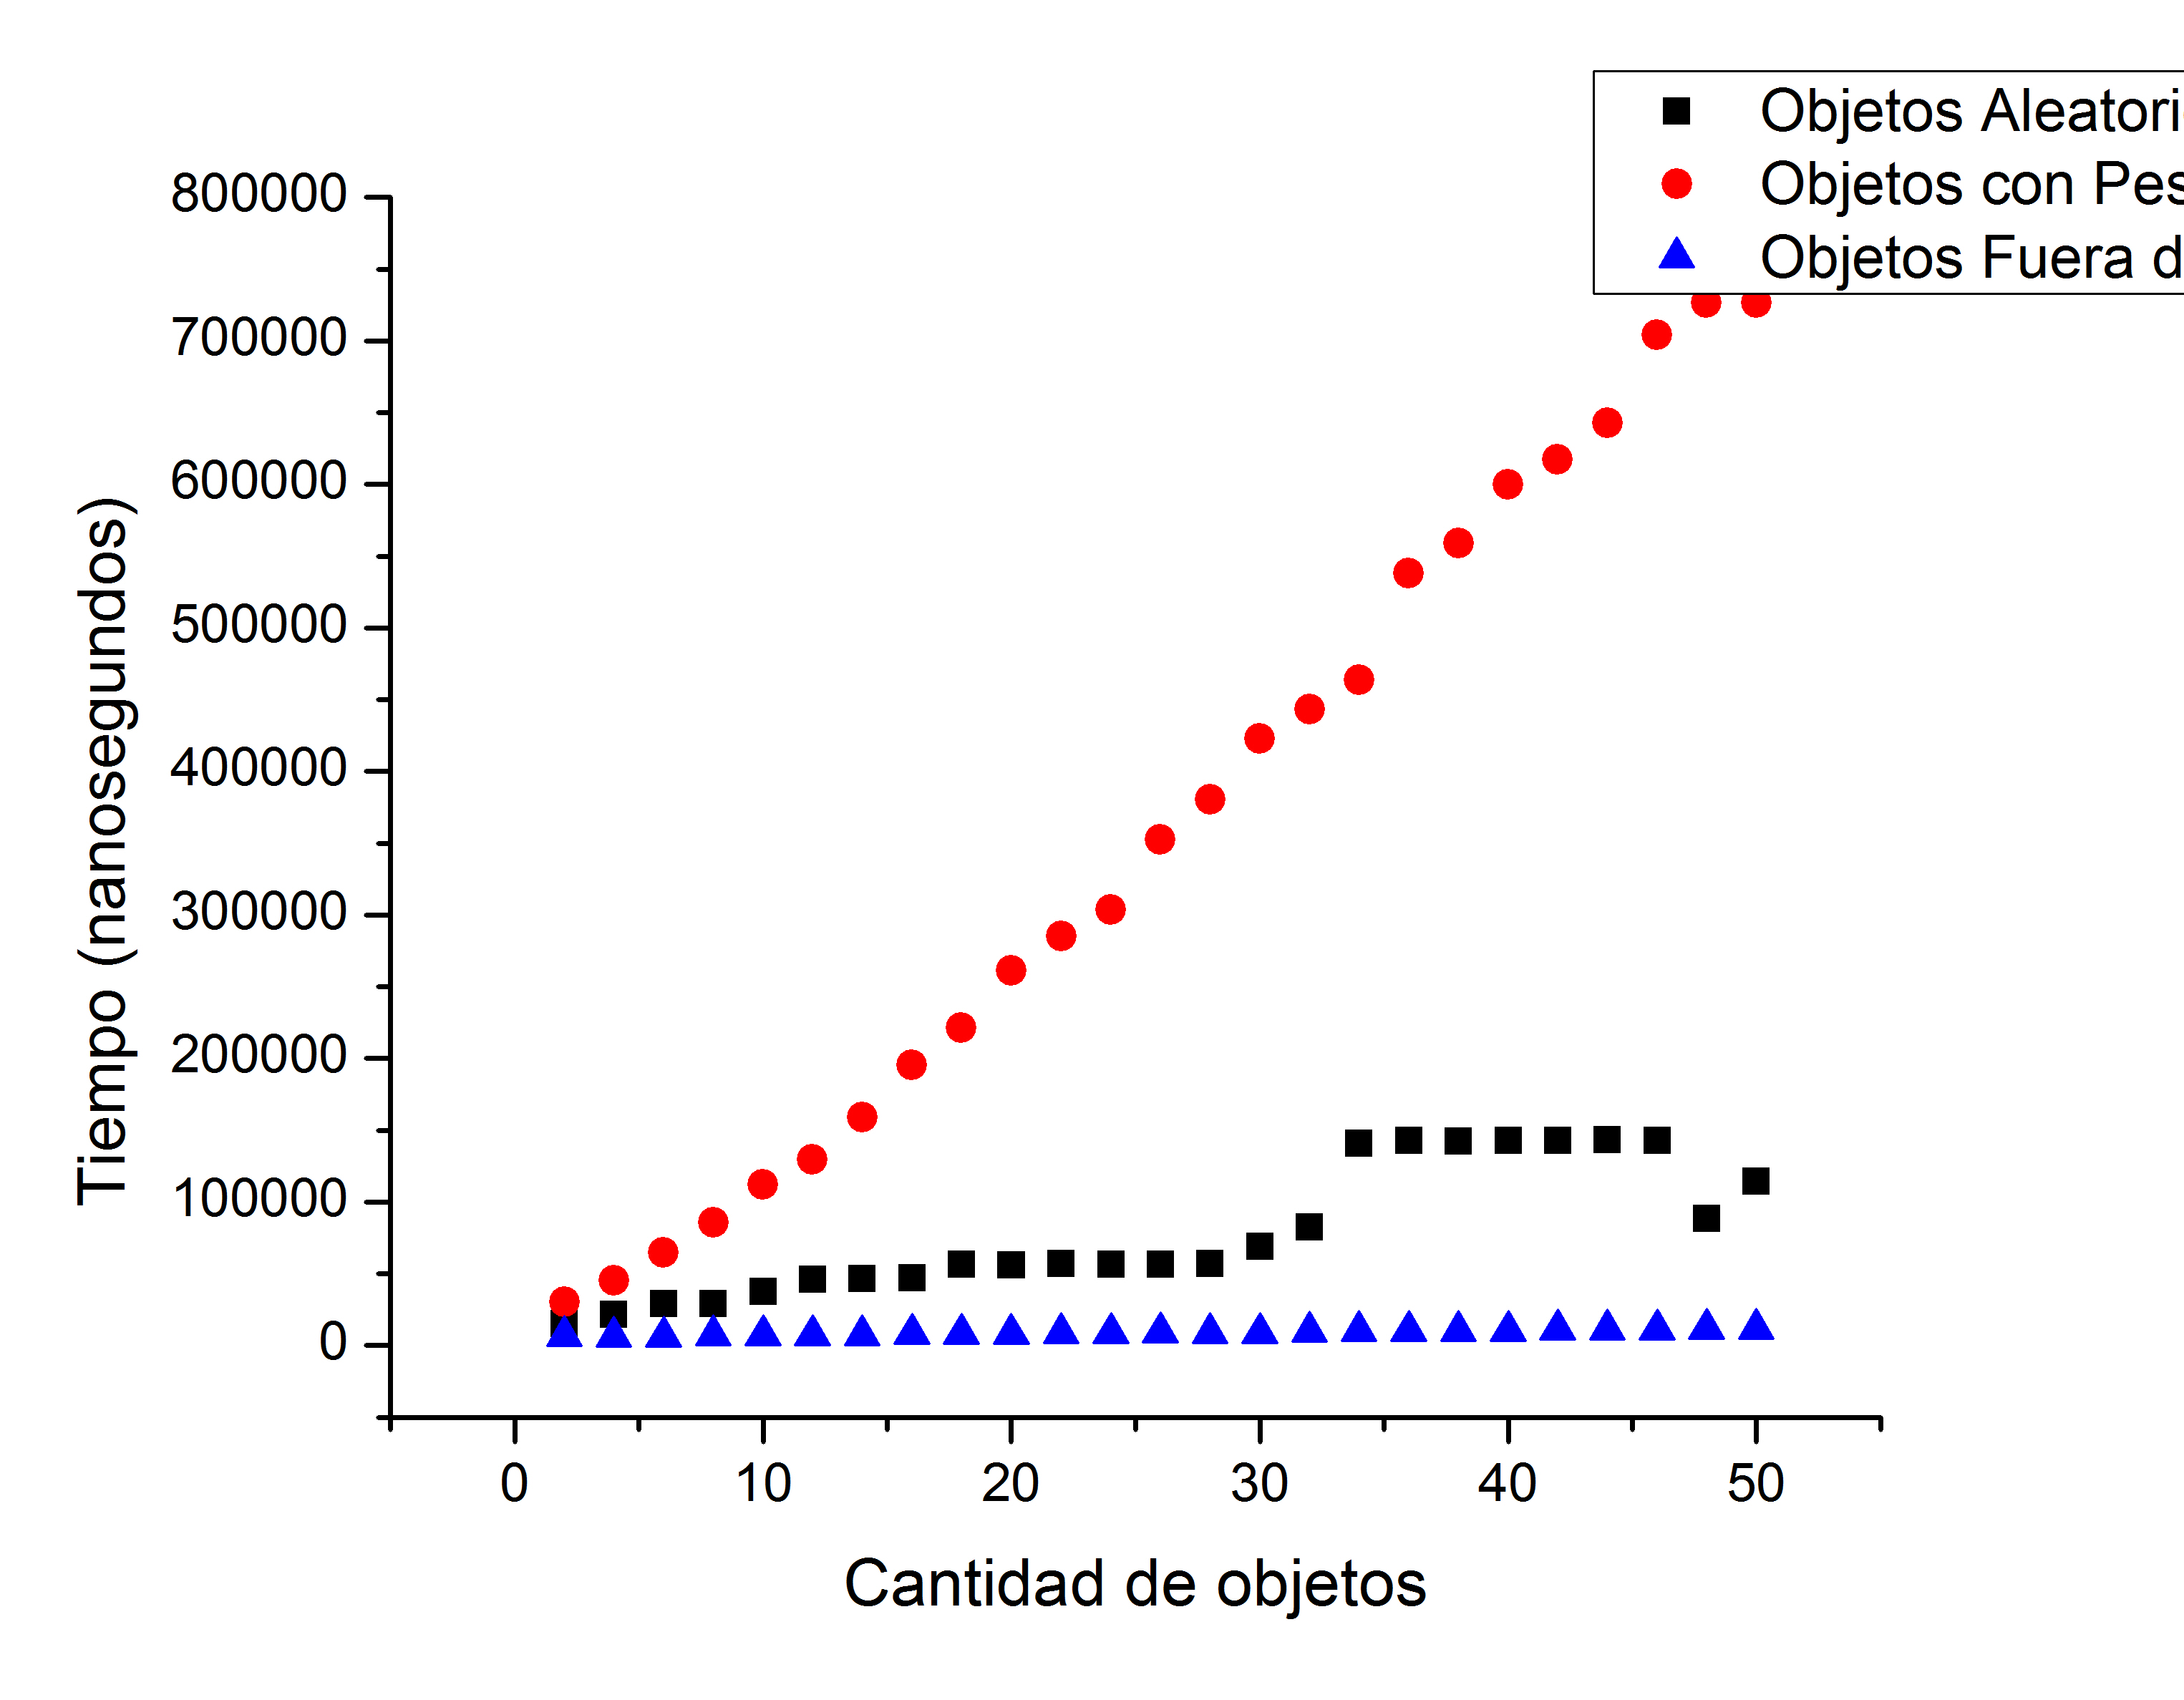
\includegraphics[width=0.6\textwidth]{comparacionObjetos}
\caption{gráfico comparativo de los tres subcasos al varias T.}
\end{figure}


En esta figura podemos observar no solo la tendencia lineal en la complejidad del algoritmo sino también la variación del crecimiento del tiempo para los distintos casos.
El hecho de que los gráficos sean lineales respaldan nuestra cota de complejidad ya que estaríamos variando el parámetro T mientras $K_1$ (la capacidad de la mochila) se mantiene constante. Estaríamos bajo la presencia de una función de tipo $Y=c*X$ con c constante.
En particular podemos destacar que en el caso de que los objetos tengan todos peso mayor a la capacidad de las mochilas, la recta tiende a ser constante y el tiempo de ejecución es casi nulo.
Podemos concluir que este sería nuestro mejor caso, y se debe al hecho de que filtramos nuestra entrada para que no se tengan en cuenta estos tesoros.
Observemos que en general lleva más tiempo obtener un resultado cuando los objetos tienen peso menor a la capacidad de la mochila.

\\
\\
\\
Luego realizamos tests para poder ver el comportamiento del algoritmo al ir aumentando el peso de la mochila. Utilizamos un test para evaluar el comportamiento cuando los objetos son aleatorios y otro para cuando todos los tesoros tienen un peso mayor a la capacidad de la mochila, en ambos casos la cantidad de objetos es constante en 50 elementos.
En esta figura podemos observar no solo la tendencia lineal de la complejidad del algoritmo sino también la variación de las pendientes en cada caso. Notemos que a mayor pendiente, la ejecución toma más tiempo, es decir es "más lenta".
En particular podemos destacar que en el caso de que los objetos tengan todos peso mayor a la capacidad de las mochilas, la recta tiende a ser constante.

\begin{figure}[H]
\centering
\includegraphics[width=0.6\textwidth]{pesoMochila}
\caption{gráfico comparativo al variar K}
\end{figure}

Podemos observar que al tener los tesoros con peso fuera del rango de la capacidad de la mochila el tiempo se mantiene constante, prácticamente nulo igual que en el experimento anterior. Con los objetos aleatorios vemos que tiene cierta tendencia lineal como es de esperarse (ya que este caso es similar al analizando en la figura()) sin embargo algunos valores quedan distorcionados. Creemos que esto se debe a que los objetos son aleatorios.
\\
\\
Finalmente corrimos tests variando la cantidad de mochilas (todas con capacidad 50) manteniendo constantes los tesoros, estos siendo 50.

\begin{figure}[H]
\centering
\includegraphics[width=0.6\textwidth]{cantMochilas}
\caption{variación de la cantidad de mochilas.}
\end{figure}

En esta figura podemos observar el crecimiento exponencial del tiempo dependiendo de la cantidad de mochilas. Esto concuerda con el hecho de que al tener todas las variables en 50 ($T=50, K_1 =50 k_2=50, k_3=50$) al ir aumentando la cantidad de mochilas estaríamos elevando la constante 50 (con $K_1$ tenemos $K_1*T=50^2$, con $K_2$ tenemos $K_1*K_2*T=50^3, etc $). Este es el tipo de función exponencial $Y=50^X$.
\\
\\
\\






:-"Y todos estos tesoros van a ir para algun museo no?"
\\
:-"Sí,Indi... lo que digas..."



\end{document}
